%%%%%%%%%%%%%%%%%%%%%%%%%%%%%%%%%%%%%%%%%
% Beamer Presentation
% LaTeX Template
% Version 1.0 (10/11/12)
%
% This template has been downloaded from:
% http://www.LaTeXTemplates.com
%
% License:
% CC BY-NC-SA 3.0 (http://creativecommons.org/licenses/by-nc-sa/3.0/)
%
%%%%%%%%%%%%%%%%%%%%%%%%%%%%%%%%%%%%%%%%%

%----------------------------------------------------------------------------------------
%	PACKAGES AND THEMES
%----------------------------------------------------------------------------------------

\documentclass{beamer}

\mode<presentation> {

% The Beamer class comes with a number of default slide themes
% which change the colors and layouts of slides. Below this is a list
% of all the themes, uncomment each in turn to see what they look like.

%\usetheme{default}
%\usetheme{AnnArbor}
%\usetheme{Antibes}
%\usetheme{Bergen}
%\usetheme{Berkeley}
%\usetheme{Berlin}
%\usetheme{Boadilla}
%\usetheme{CambridgeUS}
%\usetheme{Copenhagen}
%\usetheme{Darmstadt}
%\usetheme{Dresden}
%\usetheme{Frankfurt}
%\usetheme{Goettingen}
%\usetheme{Hannover}
%\usetheme{Ilmenau}
%\usetheme{JuanLesPins}
%\usetheme{Luebeck}
\usetheme{Madrid}
%\usetheme{Malmoe}
%\usetheme{Marburg}
%\usetheme{Montpellier}
%\usetheme{PaloAlto}
%\usetheme{Pittsburgh}
%\usetheme{Rochester}
%\usetheme{Singapore}
%\usetheme{Szeged}
%\usetheme{Warsaw}

% As well as themes, the Beamer class has a number of color themes
% for any slide theme. Uncomment each of these in turn to see how it
% changes the colors of your current slide theme.

%\usecolortheme{albatross}
%\usecolortheme{beaver}
%\usecolortheme{beetle}
%\usecolortheme{crane}
%\usecolortheme{dolphin}
%\usecolortheme{dove}
%\usecolortheme{fly}
%\usecolortheme{lily}
%\usecolortheme{orchid}
%\usecolortheme{rose}
%\usecolortheme{seagull}
%\usecolortheme{seahorse}
%\usecolortheme{whale}
%\usecolortheme{wolverine}

\setbeamertemplate{footline} % To remove the footer line in all slides uncomment this line
%\setbeamertemplate{footline}[page number] % To replace the footer line in all slides with a simple slide count uncomment this line

\setbeamertemplate{navigation symbols}{} % To remove the navigation symbols from the bottom of all slides uncomment this line
}

\usepackage{graphicx} % Allows including images
\usepackage{booktabs} % Allows the use of \toprule, \midrule and \bottomrule in tables
\usepackage{amsmath}
\usepackage{mathtools}

%----------------------------------------------------------------------------------------
%	TITLE PAGE
%----------------------------------------------------------------------------------------

\title[Short title]{Beep Beep!} % The short title appears at the bottom of every slide, the full title is only on the title page

\author{Kelsey Maass and Brisa Davis} % Your name
\institute[UW] % Your institution as it will appear on the bottom of every slide, may be shorthand to save space
{
AMATH 574 \\ % Your institution for the title page \\
Group 6
\medskip
}
\date{\today} % Date, can be changed to a custom date

\begin{document}

\begin{frame}
\titlepage % Print the title page as the first slide
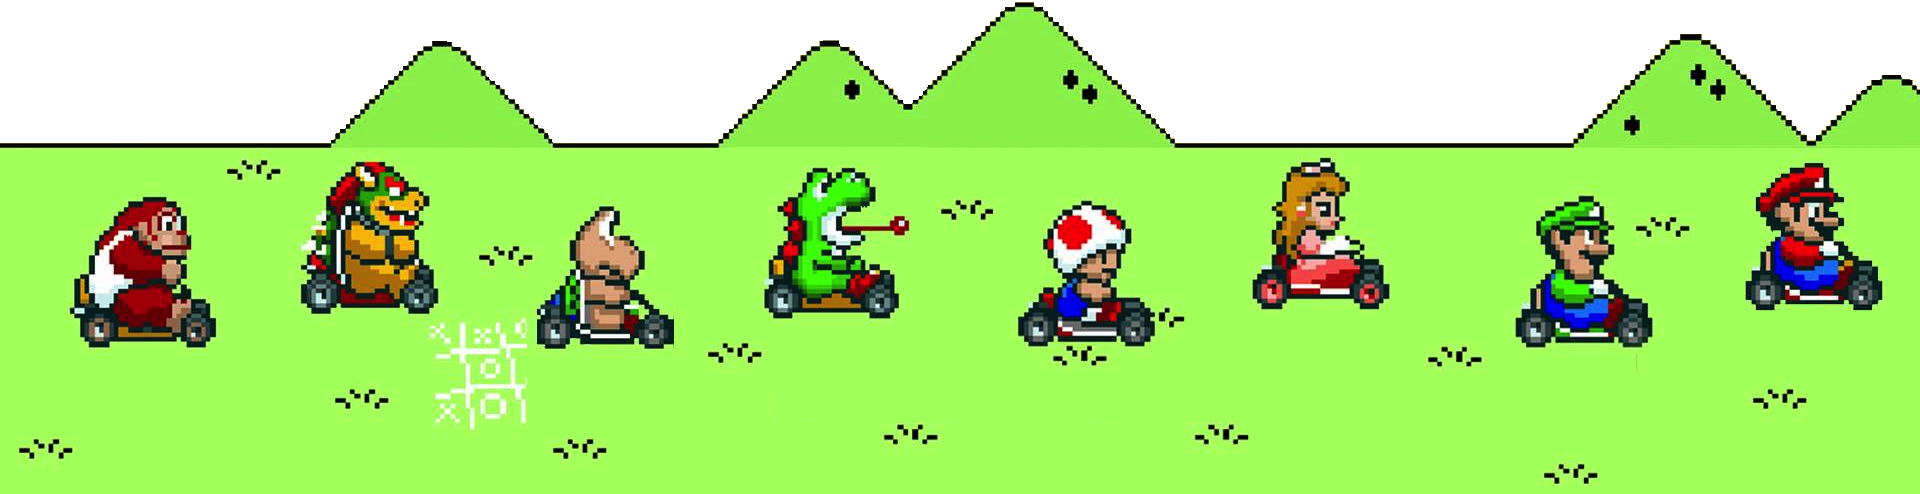
\includegraphics[width=4.75in]{mariokart.png}
\end{frame}

\begin{frame}
\frametitle{Introduction} 
\begin{itemize}
\item Are second-order models always better than first-order models?
\item Not always! The PW model for traffic flow, meant to improve the LWR model's behavior near shocks, actually performs worse than the original in some cases.
\item The PW model is based on compressible fluid dynamics, which ignores some fundamental differences between fluids and cars. Because of this, it can sometimes predict negative velocities.
\item The AR model corrects the problem of negative velocities by utilizing a convective derivative.
\end{itemize}
\end{frame}

%----------------------------------------------------------------------------------------
%	LWR Model
%----------------------------------------------------------------------------------------

\begin{frame}
\frametitle{Lighthill-Whitham-Richards (LWR) Model}

Proposed by Lighthill and Whitham (1955) and Richards (1956), the LWR model describes traffic flow on a single one-way road without entrances or exits:

\[ \rho_t + \Big(\rho V(\rho)\Big)_x = 0 \]

\begin{itemize}
\item $\rho$ = density
\item $V(\rho)$  = preferred velocity, a given nonincreasing function of $\rho$, nonnegative for $\rho$ between 0 and $\rho_m$ (the``jam" density)
\item Predicts piece-wise smooth density, with transitions between regions approximated by shocks
\item Problem: Doesn't adequately describe the motion of cars passing through shocks (cars change velocity instantaneously) 
\end{itemize}

\end{frame}

%------------------------------------------------
%	PW Model Background
%------------------------------------------------

\begin{frame}
\frametitle{Payne-Whitham (PW) Model}

Viewing traffic as a compressible fluid, Payne (1971) and Whitham (1974) introduced a second equation analogous to the conservation of momentum, $\rho v$, in fluids:

\[ \left\{ \begin{matrix*}[l] \rho_t + (\rho v)_x = 0 \\[2ex] (\rho v)_t + \Big(\rho v^2 + p(\rho)\Big)_x = 0 \end{matrix*} \right. \]

\begin{itemize}
\item $\rho$ = density
\item $v$ = velocity
\item $p(\rho)$ = ``anticipation factor", describes how a driver reacts to variations in density with respect to space
\end{itemize}

\end{frame}

\begin{frame}
\frametitle{Payne-Whitham (PW) Model}

Rewriting the second equation in terms of velocity and adding relaxation and viscosity terms, we get the full PW Model:

\[ \left\{ \begin{matrix*}[l] \rho_t + (\rho v)_x = 0 \\[2ex] v_t + v v_x + \dfrac{p'(\rho)}{\rho} \rho_x = \dfrac{V(\rho) - v}{\tau} + \mu v_{xx} \end{matrix*} \right. \]

\begin{itemize}
\item $\tau$ and $\mu$ are nonnegative constants
\item Relaxation term: represents driver's reaction time
\item Diffusion term: represents the driver's awareness of conditions ahead (and behind)
\end{itemize}

\end{frame}

\begin{frame}
\frametitle{Payne-Whitham (PW) Model}

\hspace{2em} A fundamental difference between fluids and traffic: \\[3ex]

\hspace{2em} ``A fluid particle responds to stimuli from the front and from \\ 
\hspace{2em} behind, but a car is an anisotropic particle that mostly \\
\hspace{2em} responds to frontal stimuli." CITATION

\end{frame}

\begin{frame}
\frametitle{Payne-Whitham (PW) Model}

\hspace{5em} Homogeneous model: \hspace{7em} Eigenvalues:

\[ \begin{pmatrix} \rho \\[1ex] v \end{pmatrix}_t + \begin{pmatrix} v & \rho \\[1ex] \dfrac{p'(\rho)}{\rho} & v\end{pmatrix} \begin{pmatrix} \rho \\[1ex] v \end{pmatrix}_x = 0 \hspace{3em} \lambda = v \pm \sqrt{p'(\rho)} \] \\[5ex]

From the eigenvalues we see that one characteristic speed is greater than the velocity, which means future conditions are partly determined by conditions behind. This produces an undesirable effect: negative velocities!

\end{frame}

%------------------------------------------------

%------------------------------------------------

\begin{frame}
\frametitle{PW}
Brisa, loci and integral curves. Areas of validity.
\end{frame}

%------------------------------------------------
%	AR Model Background
%------------------------------------------------

\begin{frame}
\frametitle{A thought experiment}

Consider the situation where a driver is traveling with speed $v$.  If the density ahead of him is increasing with respect to $x$ but decreasing with respect to $x - vt$, will he speed up or slow down?

\begin{figure}
\centering
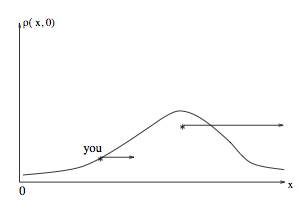
\includegraphics[width=2in]{experiment.png}
\end{figure}

\end{frame}

\begin{frame}
\frametitle{A thought experiment}

\hspace{2em} Since density ahead is increasing with respect to $x$, the PW \\
\hspace{2em} model predicts that the driver will slow down (as we will see in \\
\hspace{2em} our examples).  However, since the traffic ahead is traveling faster, \\
\hspace{2em} most drivers would actually accelerate.

\end{frame}

\begin{frame}
\frametitle{Aw-Rascle (AR) Model}

Aw and Rascle (2000) claim that instead of depending upon the derivative of pressure with respect to $x$, the anticipation factor should involve the convective derivative:

\[ \partial_t + v \, \partial_x \] \\[5ex]

This change reflects the fact that the driver's perspective is a moving frame of reference.

\end{frame}

\begin{frame}
\frametitle{Aw-Rascle (AR) Model}

Using the convective derivative, the proposed AR model is: \\[1ex]

\[ \left\{ \begin{matrix*}[l] \rho_t + (\rho v)_x = 0 \\[2ex] (v + \rho)_t + v(v + \rho)_x = 0 \end{matrix*} \right. \]

\end{frame}

\begin{frame}
\frametitle{Aw-Rascle (AR) Model}

AR model in conservation form: \\[3ex]

\[ \left\{ \begin{matrix*}[l] \rho_t + (\rho v)_x = 0 \\[2ex] \Big(\rho (v + p(\rho)) \Big)_t + \Big(\rho v(v + p(\rho)) \Big)_x = 0 \end{matrix*} \right. \] \\[5ex]

Conserved quantities:
\begin{enumerate}
\item Mass (density): $\rho$
\item ``Momentum": $y = v + p(\rho)$
\end{enumerate}

\end{frame}

\begin{frame}
\frametitle{Aw-Rascle (AR) Model}

AR model rewritten in terms of density and velocity: \\[1ex]

\[ \left\{ \begin{matrix*}[l] \rho_t + (\rho v)_x = 0 \\[2ex] v_t + \Big( v - \rho p'(\rho) \Big)_x = 0 \end{matrix*} \right. \] \\[3ex]

\hspace{5em} Linearized system: \hspace{7em} Eigenvalues:
\[ \begin{pmatrix} \rho \\[1ex] v \end{pmatrix}_t + \begin{pmatrix} v & \rho \\[1ex] 0 & v - \rho p'(\rho)  \end{pmatrix} \begin{pmatrix} \rho \\[1ex] v \end{pmatrix}_x = 0 \hspace{5ex} \begin{matrix*}[l] \lambda_1 = v - \rho p'(\rho) \\[1ex] \lambda_2 = v \end{matrix*} \] \\[1ex]

Note that neither characteristic speed is greater than the velocity!

\end{frame}

\begin{frame}
\frametitle{Aw-Rascle (AR) Model}

Aw and Rascle (2000) propose some conditions for traffic models:
\begin{enumerate}
\item The system must be hyperbolic.
\item When solving the Riemann problem with bounded nonnegative data $(\rho, v)$, the density and velocity must remain nonnegative and bounded from above.
\item When solving the Riemann problem with data $Q_{\pm} = (\rho_{\pm}, v_{\pm})$, all waves connecting any state $Q = (\rho, v)$ to its left (behind it) must have a propagation speed (eigenvalue or shock speed) at most equal to the velocity $v$.  
\item The solution to the Riemann problem must agree with the qualitative properties that each driver practically observes every day.
\item Near the vacuum, the solution to the Riemann problem must be very sensitive to the data (no continuous dependence with respect to initial data at $\rho = 0$). 
\end{enumerate}

\end{frame}

%------------------------------------------------

%------------------------------------------------

\begin{frame}
\frametitle{AR}
Brisa, loci and integral curves. Areas of validity.
\end{frame}

%------------------------------------------------

%------------------------------------------------

\begin{frame}
\frametitle{Examples}
Brisa
\end{frame}

%------------------------------------------------







\begin{frame}
\Huge{\centerline{Questions?}}
\end{frame}

%----------------------------------------------------------------------------------------

\end{document} 